\documentclass[cal1spr16Lectures.tex]{subfiles}

\begin{document}

\section[Week 10]{Week 10: 28 Mar - 1 Apr}

% % %
\subsection[4.4 Optimization Problems]{\S 4.4 Optimization Problems}
% % %

% % %
\begin{frame}{\S 4.4 Optimization Problems}
\small
In many scenarios, it is important to find a maximum or minimum value under given constraints.  Given our use of derivatives from the previous sections, optimization problems follow directly from what we have studied.
\end{frame}

% % %
\begin{frame}
\frametitle{}
\small
\begin{que} Given all nonnegative real numbers $x$ and $y$ between 0 and 50 such that their sum is 50 (i.e., $x+y=50$), which pair has the maximum product? \end{que}

\vspace{2pc}
This is a basic optimization problem.  In this problem, we are given a \alert{\bf constraint} ($x+y=50$) and asked to maximize an \alert{\bf objective function} ($A=xy$).
\end{frame}

% % %
\begin{frame}
\frametitle{}
\small
The first step is to express the objective function $A=xy$ in terms of a \alert{single variable} by using the constraint:
\[y=50-x \implies A(x)=x(50-x).\]

\vspace{2pc}
To maximize $A$, we find the critical points:
\[A^{\prime}(x)=50-2x\ \text{which has a critical point at}\ x=25.\]
\end{frame}

% % %
\begin{frame}
\frametitle{}
Since $A(x)$ has domain $[0,50]$, to maximize $A$ we evaluate $A$ \alert{at the endpoints of the domain and at the critical point}:
\[A(0)=A(50)=0\ \text{and}\ A(25)=625.\]

\vspace{2pc}
So 625 is the maximum value of $A$ and $A$ is maximized when $x=25$ (which means $y=25$).
\end{frame}

% % %
\subsubsection{Essential Feature of Optimization Problems}
% % %

% % %
\begin{frame}{\small Essential Feature of Optimization Problems}
\small
All optimization problems take the following form:
\begin{center}
\alert{\it What is the maximum (or minimum) value of an objective function subject to the given constraint(s)?}
\end{center}

\vspace{2pc}
Most optimization problems have the same basic structure as the previous problem:  An objective function (possibly with several variables and/or constraints) with methods of calculus used to find the maximum/minimum values.
\end{frame}

% % %
\begin{frame}
\frametitle{}
\small
\begin{exe} Suppose you wish to build a rectangular pen with two interior parallel partitions using 500 feet of fencing.  What dimensions will maximize the total area of the pen?
\begin{center}
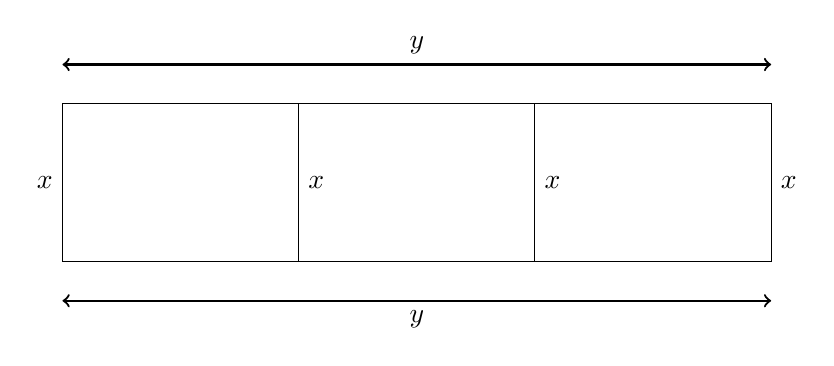
\begin{tikzpicture}
\draw (0,0) -- (3,0) 
   -- (3,2) node[midway,right] {$x$}
	 -- (0,2)
   -- (0,0) node[midway,left] {$x$};
\draw (3,0) -- (6,0)
	 -- (6,2) node[midway,right] {$x$}
	 -- (3,2)
	 -- (3,0);
\draw (6,0) -- (9,0)
	 -- (9,2) node[midway,right] {$x$}
	 -- (6,2)
	 -- (6,0);
\draw [<->] [thick] (0,-0.5) -- (9,-0.5) node[midway,below] {$y$};
\draw [<->] [thick] (0,2.5) -- (9,2.5) node[midway,above] {$y$};
\end{tikzpicture}
\end{center}
\end{exe}
\end{frame}

% % %
\begin{frame}
\small
By the picture, $2y+4x=500$ which implies $y=-2x+250$.  We are maximizing $A=xy$.  So write
\[A(x)=x(-2x+250)=-2x^2+250x.\]

Taking the derivative, $A^{\prime}(x)=-4x+250=0$, $A$ has a critical point at $x=62.5.$
\end{frame}

% % %
\begin{frame}
\footnotesize
From the picture, since we have $500$ ft of fencing available we must have $0 \le x \le 125$.  To find the max we must examine the points $x=0,62.5,125$:
\[A(\alert{0})=A(\alert{125})=0\text{ and }A(\alert{62.5})=7812.5\]

\vspace{1pc}
We see that 
\[\boxed{\text{the maximum area is}\ 7812.5\ \text{ft}^2.}\]
The pen's dimensions (answer the question!) are $\boxed{x=62.5\ \text{ft}}$ and 
\[\boxed{y=-2(62.5)+250=125\ \text{ft}.}\]
\end{frame}

% % %
\subsubsection{Guidelines for Optimization Problems}
% % %

% % %
\begin{frame}{\small Guidelines for Optimization Problems}
\footnotesize
\begin{itemize}
\item[1.] \alert{READ THE PROBLEM} carefully, identify the variables, and organize the given information with a picture.
\item[2.] Identify the objective function (i.e., the function to be optimized).  Write it in terms of the variables of the problem.
\item[3.] Identify the constraint(s).  Write them in terms of the variables of the problem.
\item[4.] Use the constraint(s) to eliminate all but one independent variable of the objective function.  
\item[5.] With the objective function expressed in terms of a single variable, find the interval of interest for that variable.
\item[6.] Use methods of calculus to find the absolute maximum or minimum value of the objective function on the interval of interest.  If necessary, \alert{check the endpoints}.
\end{itemize}
\end{frame}

% % %
\begin{frame}
\begin{que}
The sum of a pair of positive real numbers that have a product of 9 is 
\[S(x) = x + \frac{9}{x},\]
where $x$ is one of the numbers.  This sum $S(x)$ has a minimum when:
\begin{itemize}
\item[A. ] $x=9$
\item[B. ] $x=3$
\item[C. ] $x=6$
\item[D. ] none of the above
\end{itemize}
\end{que}
\end{frame}

% % %
\begin{frame}%[t]
\frametitle{}
\small
\begin{exe} An open rectangular box with square base is to be made from $48\ \text{ft}^2$ of material.  What dimensions will result in a box with the largest possible volume? \end{exe}

\vspace{1pc}
\begin{exe} Find the dimensions of the rectangle of largest area which can be inscribed in the closed region bounded by the $x$-axis, $y$-axis, and the graph of $y=8-x^3$. \end{exe}
\end{frame}

% % %
\subsubsection{Book Problems}

% % %
\begin{frame}
\begin{block}{4.4 Book Problems}
5-16, 19-20, 24, 26 
\end{block}
\end{frame}

% % %
\subsection[4.5 Linear Approximation and Differentials]{\S 4.5 Linear Approximation and Differentials}
% % %

% % %
\begin{frame}{\S 4.5 Linear Approximation and Differentials}
\footnotesize
Suppose $f$ is a function such that $f^{\prime}$ exists at some point $P$.  If you zoom in on the graph, the curve appears more and more like the tangent line to $f$ at $P$.  

\centering{\includegraphics[scale=0.54]{pictures/linApprox}}
\end{frame}

% % %
\subsubsection{Linear Approximation}
% % % 

% % %
\begin{frame}{\small Linear Approximation}
\footnotesize
This idea -- that \alert{smooth} curves (i.e., curves without corners) appear straighter on smaller scales -- is the basis of linear approximations.

\vspace{1pc}
One of the properties of a function that is \alert{differentiable} at a point $P$ is that it is \alert{locally linear} near $P$ (i.e., the curve approaches the tangent line at $P$.)

\vspace{1pc}
Therefore, it makes sense to approximate a function with its tangent line, which matches the value and slope of the function at $P$.  

\vspace{1pc}
This is why you've had to do so many ``find the equation for the tangent line to the given point" problems!
\end{frame}

% % %
\begin{frame}
\frametitle{}
\footnotesize
\begin{dfn} Suppose $f$ is differentiable on an interval $I$ containing the point $a$.  The {\bf linear approximation} to $f$ at $a$ is the linear function
\[L(x)=f(a)+f^{\prime}(a)(x-a)\qquad\text{for $x$ in $I$.}\]
\end{dfn}

\vspace{1pc}
{\bf Remarks:} Compare this definition to the following: At a given point $P=(a,f(a))$, the slope of the line tangent to the curve at $P$ is $f^{\prime}(a)$.  So the equation of the tangent line is
\[y-f(a)=f^{\prime}(a)(x-a).\]

(Yes, it is the same thing!)
\end{frame}

% % %
\begin{frame}
\frametitle{}
\small
\begin{exe} Write the equation of the line that represents the linear approximation to 
\[f(x)=\dfrac{x}{x+1}\qquad\text{ at $a=1$.}\]  
Then {\it use} the linear approximation to estimate $f(1.1)$. \end{exe}

\vspace{1pc}
{\bf Solution:} First compute
\[f^{\prime}(x)=\dfrac{1}{(x+1)^2},\quad f(a)=\dfrac{1}{2},\quad f^{\prime}(a)=\dfrac{1}{4}\]
\[L(x)=\dfrac{1}{2}+\dfrac{1}{4}(x-1)=\dfrac{1}{4}x+\dfrac{1}{4}.\]
\end{frame}

% % %
\begin{frame}
\small
{\bf Solution (continued):}

\bigskip

Because $x=1.1$ is near $a=1$, we can estimate $f(1.1)$ using $L(1.1)$:
$$f(1.1) \approx L(1.1)= 0.525$$

\bigskip

Note that $f(1.1)=0.5238$, so the error in this estimation is
$$\dfrac{0.525-0.5238}{0.5238} \times 100=0.23 \%.$$
\end{frame}

% % %
\begin{frame}
\begin{exe}
\begin{itemize}
\item[(a)] The linear approximatioln to $f(x)=\sqrt{1+x}$ at the point $x=0$ is (choose one):
	\begin{itemize}
	\item[A. ]$L(x)=1$
	\item[B. ]$L(x)=1+\textstyle\frac{x}{2}$
	\item[C. ]$L(x)=x$
	\item[D. ]$L(x)=1-\textstyle\frac{x}{2}$
	\end{itemize}
\item[(b)] What is an approximation for $f(0.1)$?
\end{itemize}
	\end{exe}
\end{frame}

% % %
\subsubsection{Intro to Differentials}
% % %

% % %
\begin{frame}{\small Intro to Differentials}
\small
Our linear approximation $L(x)$ is used to approximate $f(x)$ when $a$ is fixed and $x$ is a nearby point:
\[f(x) \approx f(a)+f^{\prime}(a)(x-a)\]

\vspace{1pc}
When rewritten,
\begin{align*}
f(x)-f(a) & \approx f^{\prime}(a)(x-a) \\[0.5pc]
\implies \Delta y & \approx f^{\prime}(a) \Delta x.
\end{align*}
\end{frame}

% % %
\begin{frame}
\footnotesize
A change in $y$ can be approximated by the corresponding change in $x$, magnified or diminished by a factor of $f^{\prime}(a)$.  

\vspace{1pc}
This is another way to say that $f^{\prime}(a)$ is the rate of change of $y$ with respect to $x$!
\begin{align*}
\Delta y & \approx f^{\prime}(a) \Delta x \\[0.5pc]
\frac{\Delta y}{\Delta x} & \approx f^{\prime}(a)
\end{align*}

\vspace{1pc}
So if $f$ is differentiable on an interval $I$ containing the point $a$, then the change in the value of $f$ (the $\Delta y$), between two points $a$ and $a+\Delta x$ in $I$, is \alert{approximately} $f'(x)\Delta x$. 
\end{frame}

% % %
\begin{frame}
\small
We now have two different, but related quantities:

\begin{itemize}
\item The change in the function $y=f(x)$ as $x$ changes from $a$ to $a+\Delta x$ (which we call $\Delta y$).

\vspace{0.5pc}
\item The change in the linear approximation $y=L(x)$ as $x$ changes from $a$ to $a+\Delta x$ (called the \alert{differential}, $dy$).
\end{itemize}

%\vspace{0.5pc}
\[\Delta y \approx dy\]
\end{frame}

% % %
\begin{frame}
\frametitle{}
\small
When the $x$-coordinate changes from $a$ to $a+\Delta x$:
\begin{itemize}
\item The function change is \underline{{\bf exactly}} $\Delta y=f(a+\Delta x)-f(a)$.
\item The linear approximation change is 
\begin{alignat*}{2}
\Delta L &= L(a+\Delta x)-L(a) \\[0.5pc]
&= \left( f(a)+f^{\prime}(a)(a+\Delta x -a) \right) - \left( f(a)+f^{\prime}(a)(a-a) \right) \\[0.5pc]
&= f^{\prime}(a) \Delta x
\end{alignat*}
and this is $dy$.
\end{itemize}
\end{frame}

% % %
\begin{frame}
\small
We define the differentials $dx$ and $dy$ to distinguish between the \alert{change in the function ($\Delta y$)} and the \alert{change in the linear approximation ($\Delta L$)}: 
\begin{itemize}
\item $dx$ is simply the change in $x$, i.e.\ $\Delta x$.
%\vspace{0.25pc}
\item $dy$ is the change in the linear approximation, which is $\Delta L=f^{\prime}(a) \Delta x$.
\end{itemize}

{\bf SO:}
\begin{align*}
\Delta L &= f^{\prime}(a) \Delta x \\[0.5pc]
dy &= f^{\prime}(a) dx \\[0.5pc]
\dfrac{dy}{dx} &= f^{\prime}(a)\quad \text{ (at $x=a$)}
\end{align*}
\end{frame}

% % %
\begin{frame}
\frametitle{}
\small
\begin{dfn} Let $f$ be differentiable on an interval containing $x$.
\begin{itemize}
\item A small change in $x$ is denoted by the {\bf differential} $dx$.
\item The corresponding change in $y=f(x)$ is \underline{approximated} by the {\bf differential} $dy=f^{\prime}(x)dx$; that is,
\begin{align*}
\Delta y& = f(x+\Delta x)-f(x) \\[0.5pc]
\approx dy &= f^{\prime}(x)dx.
\end{align*}
\end{itemize}
\end{dfn}

\vspace{1pc}
{\bf The use of differentials is critical as we approach integration.}
\end{frame}

% % %
\begin{frame}
\frametitle{}
\small
\begin{ex} Use the notation of differentials $[dy = f^{\prime}(x) dx]$ to approximate the change in $f(x)=x-x^3$ given a small change $dx$. \end{ex}

{\bf Solution:} $f^{\prime}(x)=1-3x^2$, so $dy=(1-3x^2)dx.$

A small change $dx$ in the variable $x$ produces an approximate change of $dy=(1-3x^2)dx$ in $y$.

\vspace{1.5pc}
For example, if $x$ increases from 2 to 2.1, then $dx=0.1$ and 
\[dy=\left(1-3(2)^2 \right)(0.1)=-1.1.\]
This means as $x$ increases by 0.1, $y$ decreases by 1.1.
\end{frame}

% % %
\subsubsection{Book Problems}

% % %
\begin{frame}
\begin{block}{4.5 Book Problems}
13-20, 35-50
\end{block}
\end{frame}

% % %
\subsection[4.6 Mean Value Theorem]{\S 4.6 Mean Value Theorem}
% % %

% % %
\begin{frame}{\S 4.6 Mean Value Theorem}\small
In this section, we examine the Mean Value Theorem, one of the ``big ideas" that provides the basis for much of calculus.  

\vspace{0.5pc}
Before we get to the mean Value Theorem, we examine Rolle's Theorem, where the property $f(a)=f(b)$ holds, for some function $f(x)$ defined on an interval $[a,b]$.

\begin{que}
If you have two points $(a,f(a))$ and $(b,f(b))$, with the property that $f(a)=f(b)$, what might this look like?
\end{que}
\end{frame}

% % %
\begin{frame}\small 
\begin{thm}[Rolle's Theorem]  
Let $f$ be continuous on a closed interval $[a,b]$ and differentiable on $(a,b)$ with $f(a)=f(b)$.  Then there is at least one point $c$ in $(a,b)$ such that $f^{\prime}(c)=0.$ 
\end{thm}
Essentially what Rolle's Theorem concludes is that at some point(s) between $a$ and $b$, $f$ has a horizontal tangent.
\begin{que}
Note the hypotheses in this theorem: $f$ is continuous on $[a,b]$ and differentiable on $(a,b)$.  Why are these important?
\end{que}
\end{frame}

% % %
\begin{frame}
\begin{exe}
Determine whether Rolle's Theorem applies to the function $f(x)=x^3-2x^2-8x$ on the interval $[-2,0]$.
\begin{itemize}
\item If it doesn't, find an interval for which Rolle's Thm could apply to that function.
\item If it does, what is the ``$c$" value so that $f'(c)=0$?  
\end{itemize}
\end{exe}
\end{frame}

% % %
\begin{frame}
\begin{thm}[Mean Value Theorem (MVT)]  If $f$ is continuous on a closed interval $[a,b]$ and differentiable on $(a,b)$, then there is at least one point $c$ in $(a,b)$ such that 
\[
\frac{f(b)-f(a)}{b-a}=f^{\prime}(c).
\]
\end{thm}
See Figure 4.68 on p.\ 276 for a visual justification of MVT.
\end{frame}

% % %
\begin{frame}\small  
The slope of the secant line connecting the points $(a,f(a))$ and $(b,f(b))$ is 
\[\dfrac{f(b)-f(a)}{b-a}.\]  
MVT says that there is a point $c$ on $f$ where the tangent line at $c$ (whose slope is $f^{\prime}(c)$) is parallel to this secant line.  
\begin{que}
Suppose you leave Fayetteville for a location in Fort Smith that is 60 miles away.  If it takes you 1 hour to get there, what can we say about your speed?  If it takes you 45 minutes to get there, what can we say about your speed?
\end{que}
\end{frame}

% % %
\begin{frame}%[t]
\frametitle{}
\begin{ex} Let $f(x)=x^2-4x+3.$
\begin{itemize}
\item[1.] Determine whether the MVT applies to $f(x)$ on the interval $[-2,3]$.
\item[2.] If so, find the point(s) that are guaranteed to exist by the MVT.
\end{itemize}
\end{ex}
\end{frame}

% % %
\begin{frame}%[t]
\frametitle{}
\begin{ex} How many points $c$ satisfy the conclusion of the MVT for $f(x)=x^3$ on the interval $[-1,1]$?  Justify your answer. \end{ex}
\end{frame}

% % %
\subsubsection{Consequences of MVT}
% % %

% % %
\begin{frame}{\small Consequences of MVT}
\small
\begin{thm}[Zero Derivative Implies Constant Function]
If $f$ is differentiable and $f^{\prime}(x)=0$ at all points of an interval $I$, then $f$ is a constant function on $I$.
\end{thm}

\vspace{1pc}
\begin{thm}[Functions with Equal Derivatives Differ by a Constant]
If two functions have the property that $f^{\prime}(x)=g^{\prime}(x)$ for all $x$ of an interval $I$, then $f(x)-g(x)=C$ on $I$, where $C$ is a constant.
\end{thm}
\end{frame}

% % %
\begin{frame}
\frametitle{}
\small
\begin{thm}[Intervals of Increase and Decrease]
Suppose $f$ is continuous on an interval $I$ and differentiable at all interior points of $I$.
\begin{itemize}
\item If $f^{\prime}(x)>0$ at all interior points of $I$, then $f$ is increasing on $I$.
\item If $f^{\prime}(x)<0$ at all interior points of $I$, then $f$ is decreasing on $I$.
\end{itemize}
\end{thm}
\end{frame}

% % % 
\subsubsection{Book Problems}

% % %
\begin{frame}
\begin{block}{4.6 Book Problems}
7-14, 17-24
\end{block}
\end{frame}

\end{document}